% Native editable composition from verified, unchanged IDE images.
\begin{figure}[htbp]
\centering
\sbox0{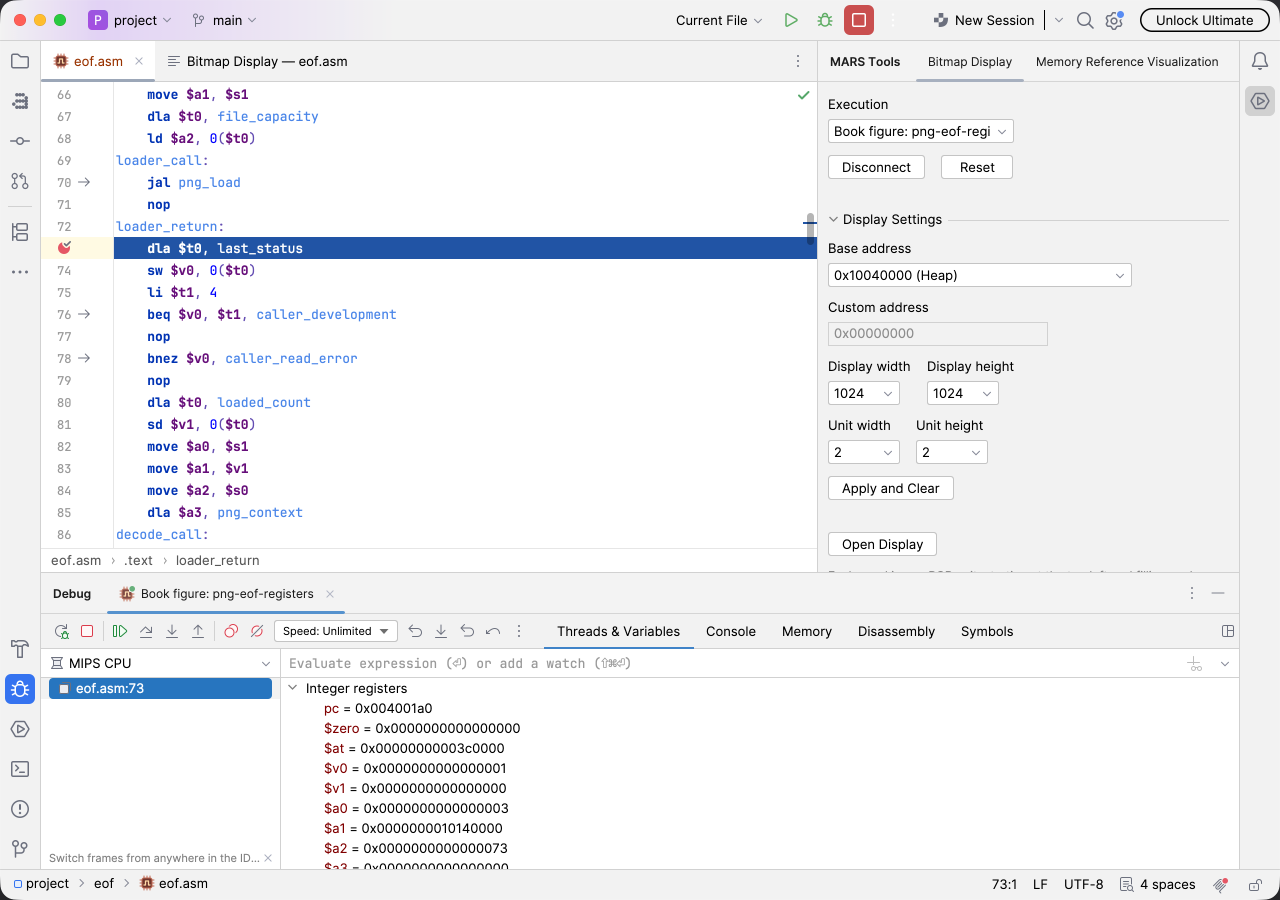
\includegraphics[artifact]{packages/033-png/captures/png-file-eof/registers.png}}
\sbox2{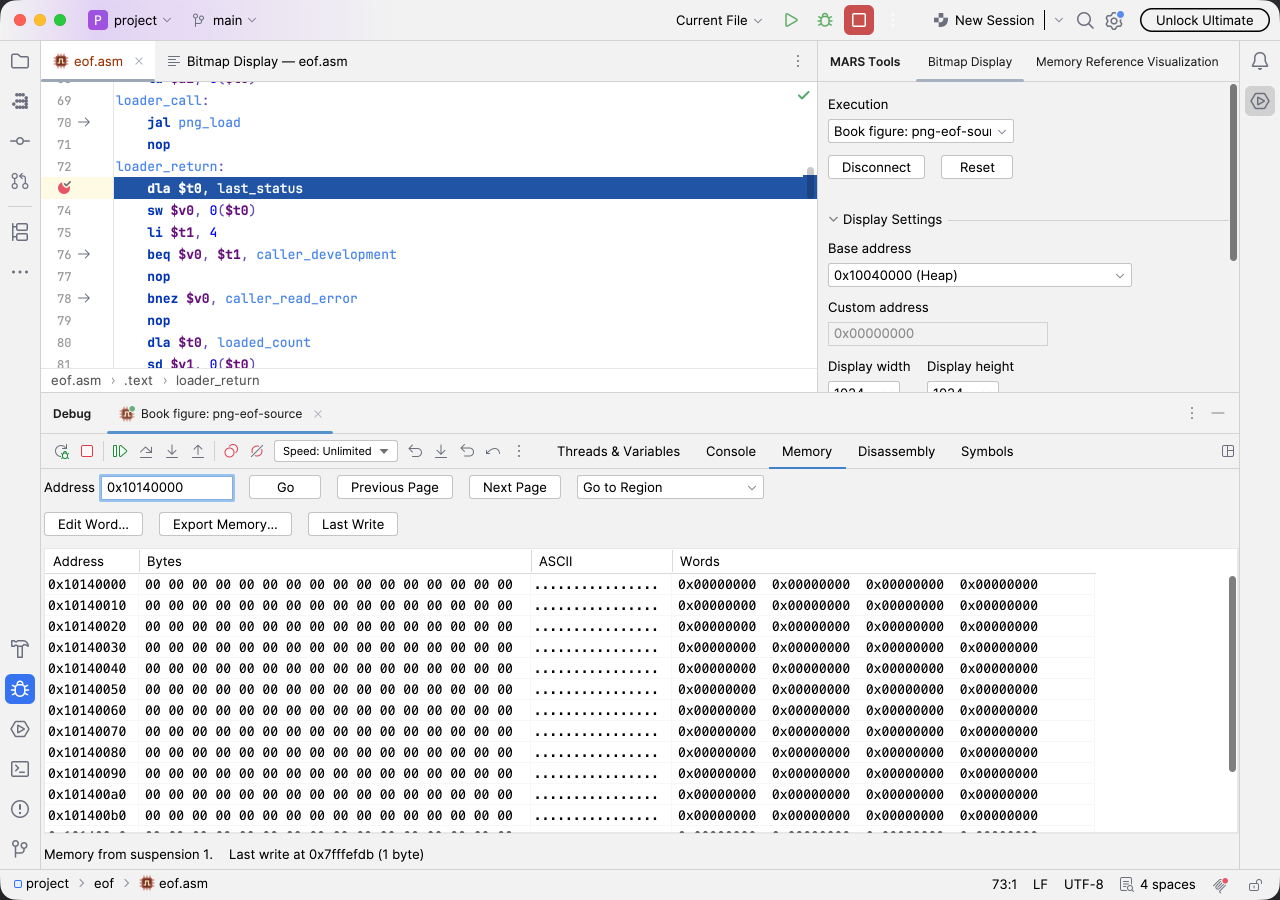
\includegraphics[artifact]{packages/033-png/captures/png-file-eof/source.png}}
\edef\MARSeofsourceLeft{\the\dimexpr0.036718750\wd0\relax}
\edef\MARSeofsourceBottom{\the\dimexpr0.707777778\ht0\relax}
\edef\MARSeofsourceRight{\the\dimexpr0.611718750\wd0\relax}
\edef\MARSeofsourceTop{\the\dimexpr0.236666667\ht0\relax}
\edef\MARSeofreturnsLeft{\the\dimexpr0.246093750\wd0\relax}
\edef\MARSeofreturnsBottom{\the\dimexpr0.110000000\ht0\relax}
\edef\MARSeofreturnsRight{\the\dimexpr0.598437500\wd0\relax}
\edef\MARSeofreturnsTop{\the\dimexpr0.838888889\ht0\relax}
\edef\MARSeofbufferLeft{\the\dimexpr0.108593750\wd2\relax}
\edef\MARSeofbufferBottom{\the\dimexpr0.335555556\ht2\relax}
\edef\MARSeofbufferRight{\the\dimexpr0.585156250\wd2\relax}
\edef\MARSeofbufferTop{\the\dimexpr0.634444444\ht2\relax}
\begin{tikzpicture}[alt={Three annotated IDE details at loader_return. The next instruction is dla t0 last_status, before the caller saves the returned status. Registers show v0 one and v1 zero. The first sixteen source-buffer bytes are zero. Independent file-service checks, rather than this photograph, establish that the acquired descriptor was closed.}]
\node[anchor=north west,inner sep=0,font=\small\bfseries] (source-title) at (6mm,0) {Returned to the supplied caller};
\node[anchor=north west,inner sep=0] (source) at ([yshift=-1mm]source-title.south west) {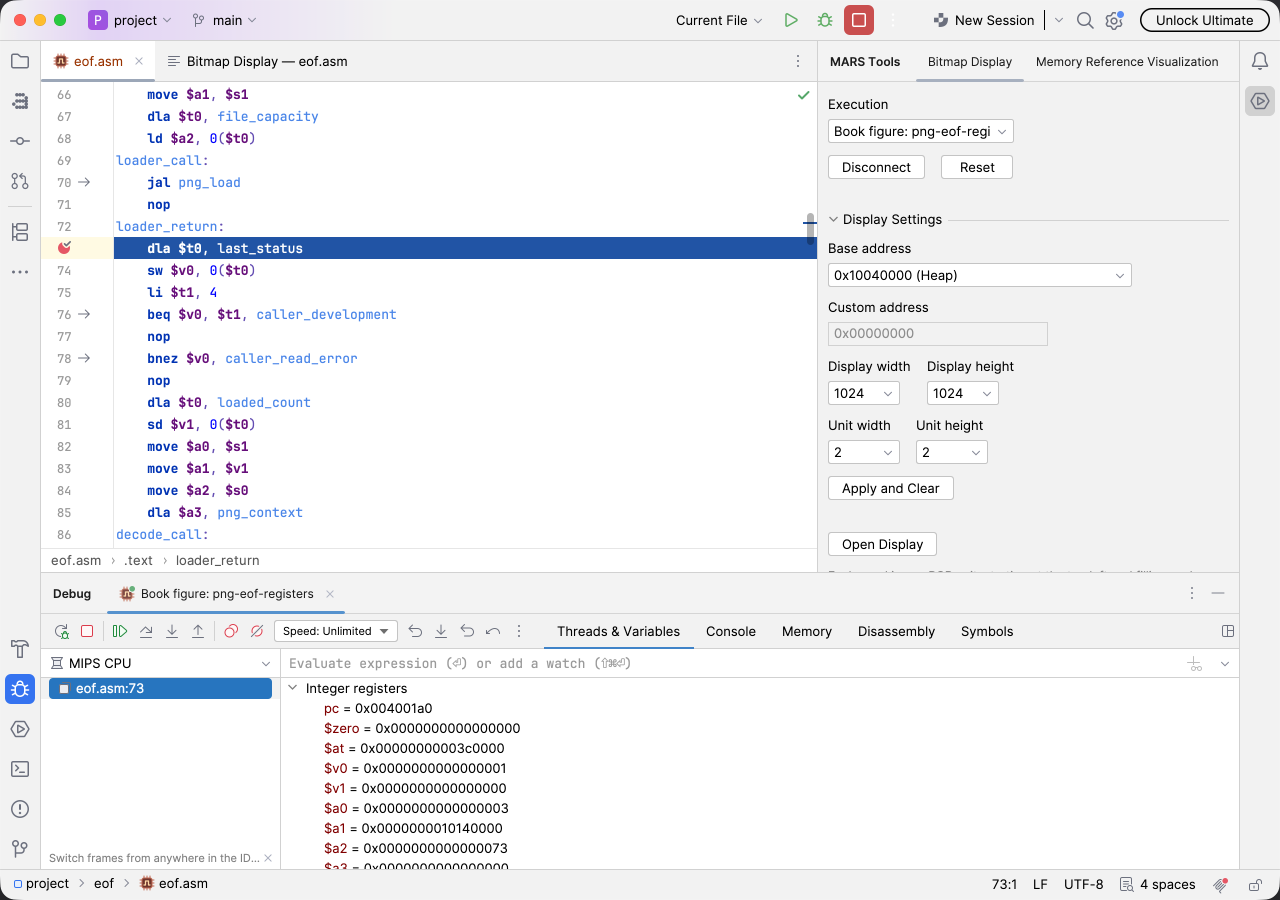
\includegraphics[width=0.7\linewidth,artifact,trim={\MARSeofsourceLeft{} \MARSeofsourceBottom{} \MARSeofsourceRight{} \MARSeofsourceTop{}},clip]{packages/033-png/captures/png-file-eof/registers.png}};
\begin{scope}[shift={(source.south west)},x={($(source.south east)-(source.south west)$)},y={($(source.north west)-(source.south west)$)}]
\draw[black,line width=0.7pt] (0.153333333,0.080000000) rectangle (0.568888889,0.520000000);
\node[draw=black,fill=white,circle,inner sep=1.5pt,font=\footnotesize] at ($(0.153333333,0.520000000)+(-3mm,0)$) {1};
\end{scope}
\node[anchor=north west,inner sep=0,font=\small\bfseries] (returns-title) at ([yshift=-2mm]source.south west) {Failure status and zero count};
\node[anchor=north west,inner sep=0] (returns) at ([yshift=-1mm]returns-title.south west) {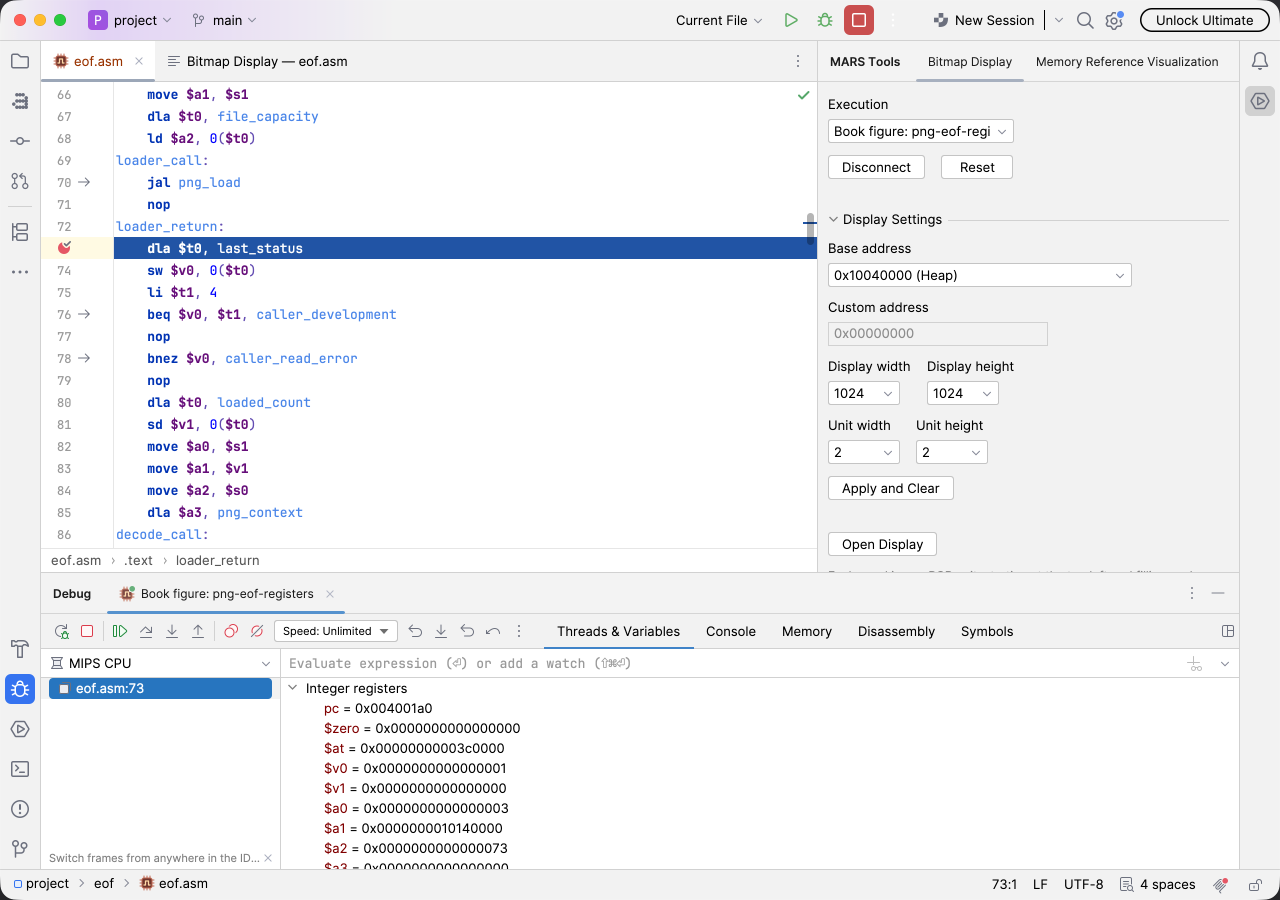
\includegraphics[width=0.5\linewidth,artifact,trim={\MARSeofreturnsLeft{} \MARSeofreturnsBottom{} \MARSeofreturnsRight{} \MARSeofreturnsTop{}},clip]{packages/033-png/captures/png-file-eof/registers.png}};
\begin{scope}[shift={(returns.south west)},x={($(returns.south east)-(returns.south west)$)},y={($(returns.north west)-(returns.south west)$)}]
\draw[black,line width=0.7pt] (0.030150754,0.065217391) rectangle (0.969849246,0.934782609);
\node[draw=black,fill=white,circle,inner sep=1.5pt,font=\footnotesize] at ($(0.030150754,0.934782609)+(-3mm,0)$) {2};
\end{scope}
\node[anchor=north west,inner sep=0,font=\small\bfseries] (buffer-title) at ([yshift=-2mm]returns.south west) {First sixteen bytes of the source buffer};
\node[anchor=north west,inner sep=0] (buffer) at ([yshift=-1mm]buffer-title.south west) {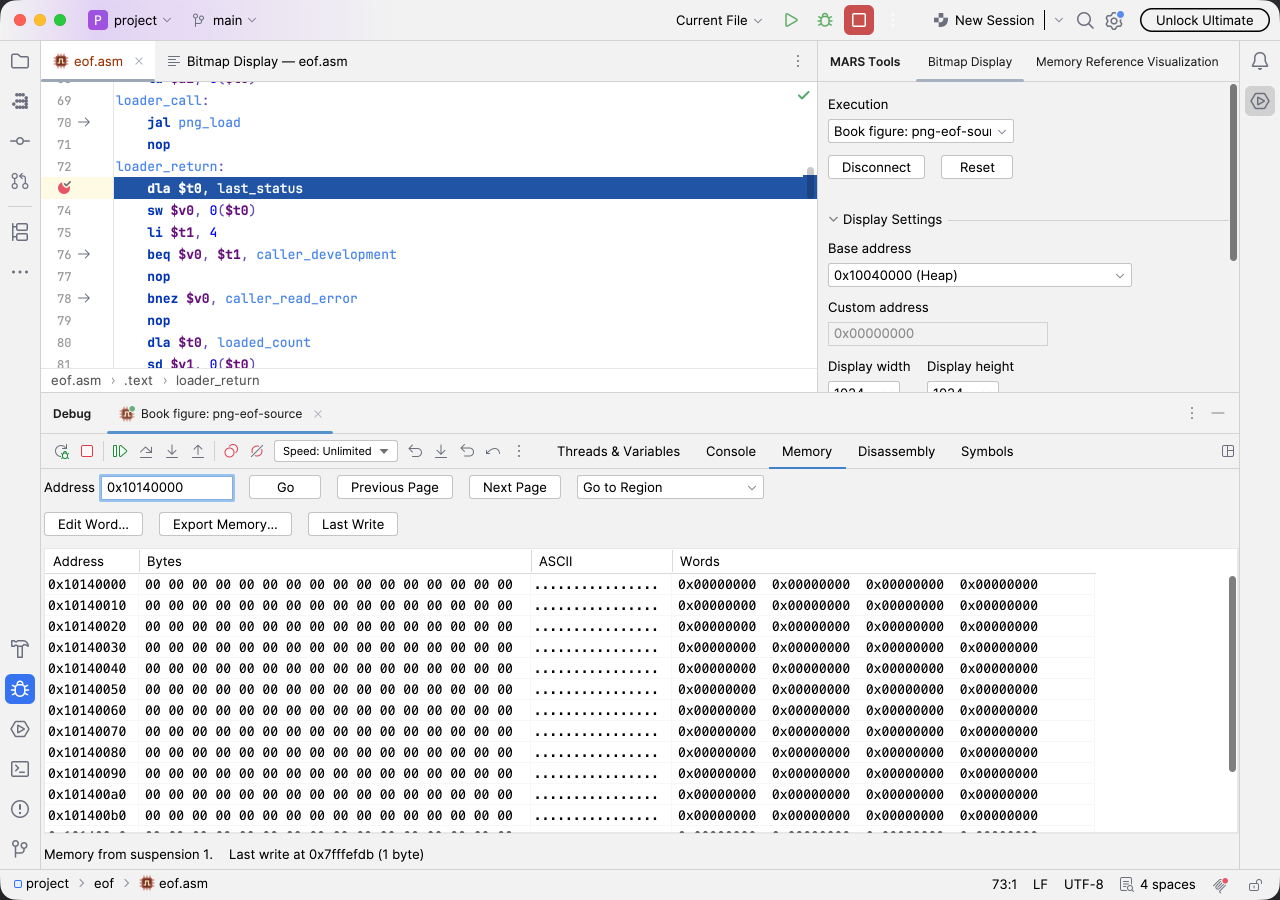
\includegraphics[width=0.82\linewidth,artifact,trim={\MARSeofbufferLeft{} \MARSeofbufferBottom{} \MARSeofbufferRight{} \MARSeofbufferTop{}},clip]{packages/033-png/captures/png-file-eof/source.png}};
\begin{scope}[shift={(buffer.south west)},x={($(buffer.south east)-(buffer.south west)$)},y={($(buffer.north west)-(buffer.south west)$)}]
\draw[black,line width=0.7pt] (0.000000000,0.111111111) rectangle (1.000000000,0.888888889);
\node[draw=black,fill=white,circle,inner sep=1.5pt,font=\footnotesize] at ($(0.000000000,0.888888889)+(-3mm,0)$) {3};
\end{scope}
\end{tikzpicture}
\par\smallskip
\begin{minipage}{\linewidth}
\small
\begin{enumerate}
\item The loader has returned. The highlighted \texttt{dla} has not yet formed the address where the caller stores its status.
\item \texttt{\$v0}=1 reports failure; \texttt{\$v1}=0 reports no loaded bytes. An empty file is rejected even though opening and reading it succeeded.
\item The source buffer remains zero in this caller. The screenshot does not establish descriptor lifetime; the independent file-service check verifies that the loader closed the descriptor.
\end{enumerate}
\end{minipage}
\caption{An empty file rejected by the loader. Two Debug launches show the same caller boundary and unchanged source buffer.}
\label{fig:png-file-eof}
\end{figure}
